\RequirePackage[orthodox]{nag}
\documentclass[11pt]{article}

%% Define the include path
\makeatletter
\providecommand*{\input@path}{}
\g@addto@macro\input@path{{include/}{../../include/}}
\makeatother

\usepackage{../../include/akazachk}

\title{Systems Identification - 111106}
\author{Andres Espinosa}
\begin{document}
\pgfplotsset{compat=1.18}
\maketitle

\tableofcontents

\section{Introduction}
\subsection{Concepts}
This course will explore a few broad topics listed below
\begin{itemize}
    \item Systems Identification
    \item State Estimation
\end{itemize}
The first section of the class will start with systems identification, we will then go over state estimation at the end.

\subsection{What is Systems Identification?}
Identifying a system deals with building a model with the goal of representation a system.
State equations, transfer functions, and frequency/step responses are mathematical ways that we can describe a system.
Graphical representations can also be useful to identify a system in a visual way.
Often, depending on the system, a photo or diagram of a system can be a useful way to extract information and gather insights.
We can also have code representations which attempt to model system logic through programmatic rules.
Physical models exist such as that of a scale representation attempts to simulate a system through simplification and minimizing the scale model of the actual system.

A dynamic system is a system that varies over time and doesn't just have an input and output but evolves over time.
On the other hand, a static system is a system that is only dependent on a transformation from its inputs to its outputs.
By building models, we can attempt to represent these systems in a few ways.
Continuous time models attempt to divide time into the true continuous time stream, where discrete times bucket time into discrete intervals.
There are also linear and nonlinear models that are used to represent systems, sometimes regardless of their linearity.

\begin{figure}[h]
\centering
\begin{tikzpicture}[>=latex, thick, node distance=2.4cm]
% Static system
\node (u_s) {$u(t)$};
\node[draw, rectangle, minimum width=1.8cm, minimum height=1.0cm, right=1.2cm of u_s] (S) {$f(\cdot)$};
\draw[->] (u_s) -- (S);
\node[right=1.2cm of S] (y_s) {$y(t)$};
\draw[->] (S) -- (y_s);
\node[below=0.25cm of S] {Static: $y(t)=f\!\big(u(t)\big)$};

% Dynamic system
\node[right=4.4cm of y_s] (u_d) {$u(t)$};
\node[draw, rectangle, minimum width=2.2cm, minimum height=1.0cm, right=1.2cm of u_d] (D) {$G$};
\draw[->] (u_d) -- (D);
\node[right=1.2cm of D] (y_d) {$y(t)$};
\draw[->] (D) -- (y_d);

% State feedback loop (memory)
\node[draw, circle, minimum size=6mm, above=1.0cm of D] (x) {$x$};
\draw[->] (x) -- (D);
\draw[->] (D) |- +(0,1.05) -| (x);

\node[below=0.25cm of D, align=center] {Dynamic: $\dot x(t)=g\!\big(x(t),u(t)\big)$\\$y(t)=h\!\big(x(t),u(t)\big)$};
\end{tikzpicture}
\caption{Static system: output depends only on present input. Dynamic system: output depends on present input and an internal state that evolves over time.}
\end{figure}

\subsection{Why Create Models?}
After creating model representations of systems, we can use the model for various reasons.
One of which is simulation. 
After creating a model, we can use a simulation to approximate and identify how a system would behave under different parameters without spending the real life physical cost associated with doing so.
We can also use a model to tune individual parameters that we have control over in the system and better design our system.
Models can also be used to design controls and vary our input parameters better.
\begin{itemize}
    \item Simulation
    \item Parameter Tuning (System Design)
    \item Controls
    \item State Estimation
    \item Fault Detection
    \item Prediction
\end{itemize}

\subsection{Models}
Different properties exist that divide models into distinct categories that inform their development and characteristics.
\begin{itemize}
    \item Discrete-time vs Continuous: Discrete timesteps $k \in \mathbb{Z}$ vs a continuous time frame $t \in \mathbb{R}$.
    \item Time-varying vs Invariant: A time-varying model has properties that change over time where as a time-invariant model does not evolve or change over time.
    \item Parametric vs Non-Parametric: A parametric model has a finite number of parameters that can be linear or non-linear.
    \item Linear vs Non-Linear: Most systems are non-linear but we can use linear models to approximate or non-linear models to attempt to model a higher degree of complexity.
\end{itemize}

\subsection{Linear Models}

\subsubsection{Box Car Example}

The system depicted in Figure \ref{fig:box_car} is a linear time-invariant system.
The spring acts with $Kp$ and the dampener counteracts it with $Cv$
\begin{equation}
    Ma = F - Kp - Cv
\end{equation}
By changing this equation where $F = u(t)$ is our input which represents our input force  and $p = y(t)$ is our output which represents the position of the car.
\begin{equation}
    M y^{\prime \prime} + C y^\prime + K y = u 
\end{equation}

\begin{figure}[h]
\centering
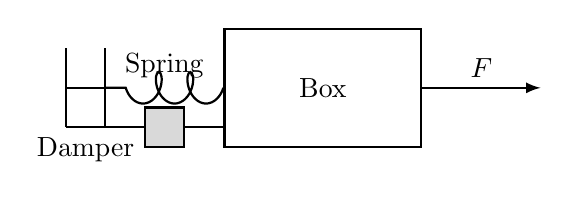
\begin{tikzpicture}[>=latex, thick, node distance=1.5cm]
% Car
\node[draw, rectangle, minimum width=2.5cm, minimum height=1.5cm] (car) {Box};

% Spring
\draw[decorate, decoration={coil, aspect=0.6, segment length=4mm, amplitude=2mm}] 
    (car.west) -- ++(-1.5cm, 0) node[midway, above] {Spring};

% Damper (parallel to spring)
\draw[thick] (car.west) ++(-1.5cm, -0.5cm) -- ++(-0.5cm, 0) 
    node[midway, below] {Damper};
\draw[thick] (car.west) ++(-1.5cm, -0.5cm) -- ++(0, 1cm);
\draw[thick] (car.west) ++(-2cm, -0.5cm) -- ++(0, 1cm);
\draw[thick] (car.west) ++(-2cm, 0) -- ++(0.5cm, 0) 
    node[midway, above] {};

\draw[thick] (car.west) ++(-2cm, -0.5cm) -- ++(2cm, 0cm);
\draw[thick, fill=gray!30] (car.west) ++(-1cm, -0.75cm) rectangle ++(0.5cm, 0.5cm);

% Force
\draw[->] (car.east) -- ++(1.5cm, 0) node[midway, above] {$F$};
\end{tikzpicture}
\caption{Box car diagram with a spring and a parallel damper on the left, and a pulling force on the right.}
\label{fig:box_car}
\end{figure}

A linear system has this equation $y(t) = y_f(t) + y_0 (t) $.
There are two special scenarios for a linear system:
One where the initial conditions are zero and we force an input to directly map to the output (forced output $y_f$),
and one where no input is ever forced into the system but the initial condition is not zero (free output $f_0$).

A property of linear systems is that, in the context of a forced output, any input can be represented as a linear combination of other inputs and the output will be the same linear combination of the corresponding outputs.

More simply, consider $x(0) = 0$ (initial state/conditions is null/zero), the following is a property of linear systems.

For a $u_1(t) \rightarrow y_1(t)$ and $u_2(t) \rightarrow y_2(t)$ and two scalars $\alpha, \beta$

\begin{equation}
    u(t) = \alpha u_1(t) + \beta u_2(t) \implies y_f(t) = \alpha y_1(t) + \beta y_2(t)
\end{equation}

\subsubsection{System Vs Model}
In the example in Figure \ref{fig:box_car}, it is easy to see that this model isn't a perfect representation of the actual system.
Friction is an important component that would introduce complexity and non-linearity.
$S = M(\theta)$ or $S=M$ means that for the purpose of the math exercise, the system is perfectly represented by its model and its parameters.

\subsubsection{Circuit Model - Nonlinear}
As an example, we can have a small system that is a battery - resistor - capacitor - ground circuit in series.

\begin{figure}[h]
\centering
\begin{circuitikz}[american]
    % Battery
    \draw (0,0) to[battery, l=$V_b(t)$] (0,2)
              to[short] (2,2)
              to[R, l=$R$] (4,2)
              to[short] (4,1)
              to[C, l=$C$] (4,-1)
              to[short] (2,-1)
              to[short] (0,-1)
              to[short] (0,0);
    % Label for capacitor voltage
    \node at (4.5, 0) {$V_c(t)$};
\end{circuitikz}
\caption{Battery-resistor-capacitor circuit in series.}
\label{fig:circuit_model}
\end{figure}

\begin{equation}
    V_b(t) = R i(t) + V_c (t)
\end{equation}
This equation can be turned into a model by having the input be the battery voltage inputted and the output be the voltage of the capacitor.
\begin{equation}
    u(t) = y(t) + RC y^\prime(t)
\end{equation}

This isn't a linear system since there will be a breaking point that will explode the capacitor if overfilled with voltage.
Although our linear model is an approximation for this more complex system, this can generally be enough for a lot of applications.
The system will frequently be "linear enough" when values are reasonably constrained or small.

\subsection{September 30th}
A transform function takes a space that it in a different domain (like time) and turns it into another domain (like complex space).
\begin{equation}
    Y_f(s) = T(s) U(s)
\end{equation}

The transfer function works with the forced output, not the free output. 
Another way to describe a transfer function is the laplace transform of the forced impulse response.
\begin{equation}
    T(s) = L \{ h(t) \}
\end{equation}

\begin{equation}
    y_f(t) = h(t) \ast u(t) = \int_{0}^{\tau} h(\tau) u(t-\tau) d \tau
\end{equation}

A system can be split into its controllable and observable parts.
A transfer function $T(s)$ works with the inputs that are both controllable and observable.
A frequency response $T(jw)$ is a transfer function that is computed in imaginary component.

\subsubsection{Plant Example}
Consider an asymptotically (it will become stable over time with any initial conditions and no input) stable plant with transfer function $G(s)$
\begin{equation}
    u(t) = \sin (wt)
\end{equation}

Since the system is asymptotically stable, after some time the free output will converge to zero and the forced output will converge to an amplified sinusoid similar to the input sinusoid.
\begin{equation}
    y_f (t) = |G(j \omega)| \sin (\omega t + \angle G(jw))
\end{equation}
where $|G(j \omega)|$ is the radius $r$ and $\angle G(jw)$ is the angle $\theta$ that the point makes with the real and imaginary plane.

\subsection{October 6th}

\subsubsection{Systems ID Types}
Black box methods of systems identification represent attempting to identify the system without information on the system's dynamics or parameters.
In order to attempt to solve it, we feed in inputs $u(t)$ and record the outputs $y(t)$ to create a dataset $D=((u_1, y_2), \dots)$.
We can identify a possible type of function, for example a rational transfer function 
\begin{equation}
    G(s) = \frac{b_m s^m + \dots + b_1 s + b_0}{a_n s^n + \dots + a_1 s + a_0}
\end{equation}

and use our dataset to attempt to fit the parameters ($a,b$) and meta-parameters ($n,m$) to the problem.

We also have a grey-box approach in which we have a known structure but we do not know the specific parameters to the system.
For example, a physics system in which we know the components in play but we do not know exact specifications like the mass or different physics constants.
We can similarly conduct experiments to attempt to parameterize the system.

Ad-hoc methods or tailor-made methods are very specific methods used to identify systems in specific domains.

\subsubsection{Frequency vs Step Response}

\subsection{October 7th}
\subsubsection{Systems Identification Process }
When we identify and build a model for a system, we typically have a goal in mind.
Our goal could be for control, estimation, diagnosis, prediction, simulation.
After we have our goal in mind for our system identification or model, we want to clarify the quantities and parameters that are entering and exiting the system.
At this point we can have a general idea of $u(t), y(t)$.
After, we want to see how much data we may have available on the system.
At times, we may only have data on the system and have little information on the system, and in other times we can only collect data through active experiments and have no previous data given such as reinforcement learning where we collect the data by running the system without access to the system itself.

A crucial choice is that of the "suitable" model class for the data and information collected.
$\mathcal{M}_n(\theta)$ is a denotion of the model class where $\mathcal{M}$ is the model class, $\theta$ is the parameters and $n$ is the complexity of the parameters. 
Typically, $\hat{\theta}$ is used as it is the estimated parameters, not the true set.
A higher degree of complexity for a parameter space naturally means that more data is needed to appropriately model the system.

Identifying the parameter vector $\hat{\theta}$ is an important task, including the complexity of the set.
After having identified the parameter vector, we must then validate and ask ourselves if we are satisfied with our model based off our data, our knowledge of the system, and some accuracy metric to characterize our proximity to satisfaction.

The following is the complete systems identification process framework
\begin{enumerate}
    \item State goal of identification
    \item Clarify inputs and outputs
    \item Identify data available (given or experiment needed)
    \item Experiment if needed and possible
    \item Choose a suitable class of models
    \item Identify the optimal parameter vector $\hat{\theta}^*$ using the data
    \item Validate and return to previosu steps as necessary
\end{enumerate}

\subsubsection{Discrete Time}
Computers don't handle continuous, so we need to give a discretized version of representations in discrete time.
We can take a continuous stream and sample them at $\Delta t$ intervals $u(t) \to u(k \Delta t) = u(k), y(t) \to y(k \Delta t) = y(k)$
For the purpose of this class, the abuse of notation we will use $u(k)\triangleq u(t=k \Delta t)$.
$u(r)$ refers to the $r$-th value in memory of the data input.

In the continuous case, when we have a $y$ output defined by $y(t) = y_f(t) + y_0(t)$, we can introduce an impulse $\delta(t)$ which pulses a property at 0 and 0 only.
We can see the impulse response $y_f(t) = h(t)$ and how the function behaves with no initial conditions and just an impulse force.

For general $u(t) \implies y_f(t) = h(t) \ast u(t) $
\begin{equation}
    h(t) \ast u(t) = \int_{0^-}^{t} h(\tau) u(t-\tau) d \tau
\end{equation}
To relate using the laplace transformed input we have
\begin{equation}
    Y_f (s) = G_c (s) U(s)
\end{equation}
where $G_c(s) = \mathcal{L}\{ h(t) \}$

In the case of discrete-time, we can rewrite and redefine these properties in discrete time step $k$.
\begin{equation}
    \delta (k) \triangleq 
    \begin{cases}
        1 & k = 0 \\ 0 & k \neq 0
    \end{cases}
\end{equation}
for this impulse, $f_f(k) = h(k)$.

For a generalized input $u(k)$,
\begin{equation}
    y_f(k) = \sum_{l = 0}^k g(l) u(k-l)
\end{equation}

\subsection{October 13th}
When we have discrete time, it can be modeled as discrete time where the input occurs as impulses at every $k$-th timestep.
The forced output is therefore
\begin{equation}
    y_f(k) = \sum_{l=0}^{K} g(l) u(K-l)
\end{equation}
In the event that $K=\infty$, there is no initial condition and then
\begin{equation}
    y(k) = y_f(k) = \sum_{l=0}^{\infty} g(l) u(K-l)
\end{equation}

Given a sequence of values $v(k), k=0,1,2,\dots$, we can define a Z-transform $V(z) \triangleq \sum_{k=0}^{\infty} v(k) Z^{-k}$.
Additionally, given that sequence of $v(k)$, we can define a one-step of delay operator as $z^{-1}$, where
\begin{equation}
    z^{-1} v(k) = v(k-1)
\end{equation}
delays the sequence of values by one timestep. 
Effectively, this operator will shift a signal by one timestep.
Naturally, this operator can be extended to shift the signal by any timestep $l$.
\begin{equation}
    z^{-l} v(k) = v(k-l)
\end{equation}
We can therefore rewrite the forced output $y_f(k)$ with this new delay operator
\begin{equation}
    y_f(k) = \sum_{l=0}^{\infty} g(l) z^{-l} u(k) =  (\sum_{l=0}^{\infty} g(l) z^{-l}) u(k) = G(z) u(k)
\end{equation}
where $G(z)$ is an operator that is the z-transform of the $g(k)$ impulse reponse sequence.
This z-transform $G(z)$ is also called the transfer function and can be interpreted as an operator.
This means that $G(z) u(k) = [g(0) + g(1) z^{-1} + \dots] u(k) = g(0) u(k)+ g(1) z^{-1} u(k) + \dots$.
To show that the $G(z)$ isn't the complex domain we can change the notation to be $G(q)$.

Consider some systems that have an input $u(k)$, a transfer function $G(z)$, and a forced output $y_f(k)$.
If the system experiences an impulse response of the impulse, that means the transfer function $\mathcal{L}\{ \delta(k) \} = 1$ and the forced output is $y_f(k) = u(k)$.
If the system experiences an impulse response of the delay, that means the transfer function $\mathcal{L}\{ z^{-1} \}$ and the forced output is $y_f(k) = u(k-1)$.

An anti-transform is taking a $G(z)$ to $g(z)$.
We can do this by understanding the functions that can comprise the impulse responses in discrete time.
\begin{gather}
    G(z) = \frac{z}{z+1} = 1 - \frac{1}{z+1} \\
    = 1 - z^{-1} + z^{-2} - z^{-3} + z^{-4} + \dots
\end{gather}
This is an oscillating step function with values (+1) for any odd steps and (-1) for any evens.
Similarly we can do $G(z) = \frac{z}{z-1}$ and find the heaviside step function.

\subsubsection{Exercise Z anti-transform}
\begin{gather}
    G(z) = \frac{z}{z-1/2} = 1 + \frac{1/2}{z-1/2} \\
    = 1 + \frac{1}{2} z^{-1} + (\frac{1}{2})^2 z^{-2} + \dots
\end{gather}

By putting rational transfer functions into a form that has only negatives, it makes it easy to do the anti-transform.
In the event that the degree of the numerator exceeds that of the denominator, then the system is not a causal system.
\begin{equation}
    G(z) = \frac{b_m z^m + b_{m-1} z^{m-1} + \dots + b_0}{a_n z^{n} + a_{n-1} z^{n-1} + \dots + a_0}
\end{equation}

\subsection{October 20th}
When we introduce a non-controllable variable $n(k)$, we then have a system equation containing this observable disturbance.
\begin{equation}
    y(k) = G(z) u(k) + H(z) n(k) = \frac{B(z)}{A(z)} u(k) + \frac{D(z)}{C(z)} n(k)
\end{equation}
The variable $n$ belongs to a white noise space $n(k) ~ WN(\sigma, \lambda^2)$.
A white sequence means that any single point has no correlation with other points over time in the future or past.
A memoryless property or no memory in a sequence means that that sequence is white.

Ergodicity is a property that says that the average of collected signal data approaches the real signal average.

In order to have a causal system, for $G(z)= \frac{B(z)}{A(z)}$ we need the following:
\begin{equation}
    A(z) = 1 + a_1 z^{-1} + a_2 z^{-2} + \dots + a_n z^{-n}
\end{equation}
and
\begin{equation}
    B(z) = b_0 + b_1 z^{-1} + \dots + b_m z^{-m}
\end{equation}

where $a_0 = 1$ and $b_0 \in \mathbb{R}$ guarantees that the degree of the denominator is greater than or equal to that of the numerator.
The case is different for the disturbance $H(z) = \frac{D(z)}{C(z)}$.
We can assume that both $D,C$ are monic (they have $d_0, c_0 = 1$)
This is due to the fact that $H$ is a white noise function and therefore has a zero mean.

We can then create a parameter vector $\theta$ that parametrizes the "true" system.
\begin{align}
  \theta = 
  \begin{bmatrix}
    a_1 \\ \vdots \\ a_n \\ b_0 \\ \vdots \\ b_m \\ c_1 \\ \vdots \\ c_l \\ d_1 \\ \vdots \\ d_q
  \end{bmatrix}
\end{align}
and $p$ is the total dimension $n+m+1+l+q$.

In the system identification framework, our goal is to approximate this true parameter set that defines our underlying system.
We create a model that has an estimated parameter vector $\hat{\theta}$.
We want to drive both our model's parameters $\hat{\theta}$ to optimality and the complexity of the model itself $p$.
This optimal solution in both values and complexity is denoted $\hat{\theta}_{p^*}^*$

\subsection{October 21st}
When we predict the next output $y(k+1)$ using the form with controllable inputs $u$ and uncontrollable interferences $n$, 
\begin{equation}
    y(k) = \frac{B(z)}{A(z)} u(k) + \frac{D(z)}{C(z)} n(k)
\end{equation}
we use all previous outputs and inputs $y, u$ to predict $y(k+1)$.
In the event that $b_0 \neq 0$, we also use the future input $u(k+1)$ to predict the future output.
Therefore, given an information set $I$ at a moment $k$, we want to predict the future output.
\begin{equation}
    E[y(k+1) | I(k)]
\end{equation}.
We can bring in the estimated parameter vector to create a representation of our predicted output at a moment $k$.
\begin{equation}
    \hat{y} (k | \hat{\theta}) = E[y(k) | I(k-1)]
\end{equation}

where the information set $I$ is 
\begin{equation}
    I(k-1) = 
    \begin{cases}
       u(0), \dots, u(k) \\
       y(0), \dots, y(k-1)
    \end{cases}
\end{equation}

Although you would think that would mean we can get rid of the noise because the expectation of $n(k)$ is zero, but we can not do that.
Our previous interferences and white noise has an effect on our information set $I$.
Since $C,D$ are monic, we can invert that transfer function and move the equation around.
\begin{gather}
    \frac{C}{D}y(k) = \frac{C B}{D A} u(k) + n(k)\\
    (1-1 \frac{C}{D}) y(k) = \dots \\
    y(k) = [1-\frac{C}{D}]y(k) + \frac{C B}{D A} u(k) + n(k)
\end{gather}
The bottom equation is called the model in prediction form.
We can handle the y(k) on the right side in the following way using the fact that both $C,D$ are monic functions:
\begin{gather}
    [1-\frac{C}{D}]y(k) = [1-1 - \alpha_1 z^{-1} - \alpha_2 z^{-2} - \dots] y(k) \\
    = -\alpha_1 y(k-1) - \alpha_2 y(k-2) - \alpha_3 y(k-3) - \dots
\end{gather}
\begin{equation}
    \hat{y}(k|\theta) = [1- \frac{C(z)}{D(z)}]y(k) + \frac{C(z) B(z)}{D(z) A(z)} u(k)
\end{equation}

Where the error between this prediction and the actual system logic is
\begin{equation}
    e(k|\theta) = y(k) - \hat{y}(k|\theta) = n(k)
\end{equation}

\begin{equation}
    \hat{y} (k | \theta) = [z \frac{D(z) - C(z)}{D(z)}] y(k-1) + \frac{C(z) B(z)}{D(z) A(z)} u(k)
\end{equation}

\subsection{October 27th}
In the event that we have no noise and an ideal case, we can clearly rearrange a system with transfer functions
\begin{equation}
    A(z) y(k) = B(z) u(k)
\end{equation}
this ideal case is generally never true, and instead we have some error and the following equation
\begin{equation}
    A(z) y(k) - B(z) u(k) = \epsilon (k)
\end{equation}
where $\epsilon$ represents the error in the model.
Since $\epsilon$ can be anything, this equation-error model is always true.

Ideally, we have a small white noise that can parametrize our error and therefore $\epsilon(k) = n(k)$.
\subsubsection{ARX Model}
The ARX model is the following
\begin{equation}
    A(z) y(k) = B(z) u(k) + n(k)
\end{equation}
where the predicted output is a linear combination of the previous outputs, all inputs and the disturbances.
This is a regression on the same quantities, therefore it is an auto regressive as it incorporates the previous values of $y$.
\begin{equation}
    y(k) = -a_1 y(k-1) - \dots - a_m y(k-m) + b_0 u(k) + \dots + b_m u(k-m) + n(k)
\end{equation}
This is an autoregressive and exogenous input model.
\begin{equation}
    y(k) = \frac{B(z)}{A(z)} u(k) + \frac{1}{A(z)} n(k)
\end{equation}
Rearranging in the above equation shows that this holds the general form with $D(z) = 1, C(z) = A(z)$.
\begin{equation}
    y(k) = [1-A(z)] y(k) + B(z) u(k) + n(k)
\end{equation}
The above equation is the ARX model in predictive form.
We can put this into a glorious matrix/vector form by putting the outputs and inputs into a single vector
\begin{align}
\phi(k) =
  \begin{bmatrix}
     -y(k-1)  \\ \vdots \\ -y(k-n) \\ u(k) \\ \vdots \\ u(k-m)
  \end{bmatrix}
\end{align}

and the linear coefficients

\begin{align}
    \theta = 
  \begin{bmatrix}
     a_1 \\ \vdots \\ a_n \\ b_0 \\ \vdots \\ b_m
  \end{bmatrix}
\end{align}

\begin{equation}
    y(k) = \phi(k)^\top \theta + n(k)
\end{equation}

We can create models that incorporate a linear combination (a moving average) of the disturbances.
\begin{equation}
    y(k) = -a_1 y(k-1) - \dots - a_n y(k-n) + b_0 u(k) + \dots + b_m u(k-m) + n(k) + d_1 n(k-1) + \dots d_q n(k-q)
\end{equation}
This represents the ARMAX model (AutoRegressive eXogenous input Moving Average).
This occurs when $C(z) = A(z)$ but there is a unique $D(z)$ that we can model.
This means that the noise is not necessarily white noise.
In the event that the noise is white, we have the ARX model, however if there is some structure or correlation of the noise with previous values then we have the ARMAX model.

\begin{equation}
    y(k) = [1-\frac{A(z)}{D(z)}] y(k) + \frac{B(z)}{D(z)} u(k) + n(k)
\end{equation}
this above equation is the predictive form of the ARMAX model.
Now, we have parameters in the denominator so the predictive form is not linear in the parameters $\theta$ as it was in the ARX model.

As we have our defining polynomials $A(z), B(z), C(z), D(z)$, we have $n,m,l,q$ unknowns as well as not actually knowing what $n,m,l,q$ are.
In order to identify our system and get information such that we can make decisions about our model, parameters, and meta-parameters we can create an experiment to build a dataset.
\begin{equation}
    \{ (u(r), y(r)), r = 1,2,\dots,N \}
\end{equation}
We use the dataset that was collected offline to build an estimate of the parameters $\hat{\theta}$.


\section{EXTRA: Systems and Signals}
\subsection{Background}
\subsubsection{Complex Numbers}
Electrical engineers use the notation $j$ instead of $i$ for complex numbers.

\begin{equation}
    j^2 = -1 \quad \text{and} \quad \sqrt{-1} = \pm j
\end{equation}

Since $e^{j \theta} = \cos \theta + j \cos \theta$, we can have a polar representation of complex numbers as $z = re^{j \theta}$.
We also have the following facts that allow us to move between the forms and express in both polar and rectangular forms.
\begin{itemize}
    \item $a = r \cos \theta \quad b = r \sin \theta$
    \item $r = \sqrt{a^2 + b^2} \quad \theta = \tan^{-1} (\frac{b}{a}) $
\end{itemize} 

We can also represent the magnitude of $|z|$ as the radius $r$ which is the distance of the point $z$ from the origin.
The angle $\theta$ can similarly be represented as $\angle z$.

The conjugate $z^*$ of a complex number $z=a+jb$is defined as 
\begin{equation}
    z^8 = a - jb = re^{-j \theta},
\end{equation}
which is a mirror image of $z$ about the horizontal (real) axis.
We can easily see that the sum of a complex number and its conjugate is a real number equal to twice the real part of the number:
\begin{equation}
    z + z^* = (a+jb) + (a-jb) = 2a,
\end{equation}
and the difference of a complex number and its conjugate is an imaginary number equal to twice the imaginary part of the complex number:
\begin{equation}
    z - z^* = (a+jb) - (a-jb) = 2jb.
\end{equation}

The product of the two is the square of the magnitude
\begin{equation}
    zz^* = (a+bj)(a-bj) = a^2 -(jb)^2 = a^2 + b^2 = |z|^2.
\end{equation}

In simpler terms, $re^{j\theta}$ represents a point $z$ that has a distance $r$ from the origin and an angle $\theta$ with the horizontal axis.

When adding or subtracting complex numbers, the cartesian form is preferred due to its simplicity.
Conversely, for multiplying, dividing, or raising to a power, the polar form simplifies greatly compared to the cartesian form.

\subsubsection{Sinusoids}
For a sinusoid $x(t) = C \cos (2\pi f_0 t + \theta)$, we know that the sinusoid repeats itself every $2\pi n$ where $n \in \mathbb{Z}$.
The section $f_0 t$ is an integer whenever $t$ changes by $1/f_0$.
Commonly, $f_0$ is known as the frequency and $T_0 = \frac{1}{f_0}$ is known as the period.
$C$ is the amplitude and $\theta$ is the phase.

The variable $w_0$ is used frequently (radian frequency) to express $2\pi f_0$.
$w_0$ has units in radians whereas $f_0$ has units in hertz.
This leads to the following sinusoid representation
\begin{equation}
    x(t) = C \cos (w_0 t + \theta)
\end{equation}
where the the period $T_0 = \frac{2 \pi}{w_0}$.

\begin{figure}[htbp]
  \centerline{\includegraphics[width=0.75\textwidth]{../../images/example_sinusoids.png}}
  \caption{Some examples of different sinusoids}
  \label{fig:example_sinusoids}
\end{figure}

It is important to remember that getting from $\sin$ to $\cos$ is as simple as shifting by $\pi/2$
\begin{equation}
    C \cos(w_0 t - \pi/2) = C \sin w_0 t
\end{equation}

$\sin w_o t$ lags $\cos w_0 t$ by $\pi/2$.

We can add two sinusoids that have the same frequency easily.

\begin{equation}
    C \cos \theta \cos w_0 t - C \sin \theta \sin w_0 t = C \cos (w_0 t + \theta) = a \cos w_0 t + b \sin w_0 t 
\end{equation}

\subsubsection{Exponentially-Decaying Sinusoids}
An exponentially-decaying sinusoid has the form 
\begin{equation}
    Ae^{-at} \cos (\omega_0 t + \theta)
\end{equation}
\begin{figure}[htbp]
  \centerline{\includegraphics[width=0.75\textwidth]{../../images/drawing_exponential_sinusoids.png}}
  \caption{An example of combining an exponential and sinusoid into an exponentially-decaying sinusoid.}
  \label{fig:drawing_exponential_sinusoids}
\end{figure}

\subsubsection{Cramer's Rule}
A linear equation with the same amount of equations and unknowns $n$ can be solved with Cramer's Rule.
\begin{equation}
    x_k = \frac{|\textbf{D}_k|}{|\textbf{A}|} \quad k = 1,2,\dots, n
\end{equation}
This only occurs if the determinant of \textbf{A} is not zero and is therefore non-singular.

\subsubsection{Partial Fraction Expansion}
If we have a function that is a fraction of two polynomials, this function $F$ is improper if $m$ (the degree of the numerator polynomial) is larger than $n$ (the degree of the denominator).
It is proper if the converse holds.
\begin{equation}
    F(x) = \frac{P(x)}{Q(x)} = \frac{b_m x^m + b_{m-1} x^{m-1} + \dots + b_1 x + b_0}{a_n x^n + a_{n-1} x^{n-1} + \dots + a_1 x + a_0}
\end{equation}
An improper fraction can always be turned into the sum of a polynomial and a proper fraction ($m < n$).
There are a few ways that we can turn a rational function $F(x)$ into partial fractions.
Clearing fractions can be used by splitting into each partial fraction with their root denominators and then multiplying to remove fractions, and finally solving a system of equations.
The method of residues involves getting to a set of factors that are distinct for $Q(x)$ and then plugging them into the original $F(x)$ while excluding that root from the equation.

\section{Ljung Systems Identification}
\subsection{Introduction}
\subsubsection{Dynamic Systems}
A system is some kind of object that interact with and produce signals.
An input $u$ enters the system that is controllable by the user alongside a set of uncontrollable but observable inputs $w$.
There are additional disturbances that influence the system but are not observable or controllable $v$.


\end{document}